%\newcounter{keepage}
%\setcounter{keepage}{\value{page}} % uložíme aktuální číslo
%\pagenumbering{gobble}
%
%
%\clearpage
%\pagenumbering{arabic}
%\setcounter{page}{\value{keepage}} % vrátíme 28
%\addtocounter{page}{}             % posuneme na 29

%%%%%%%%%%%%%%%%%%%%%%%%%%%%%%%%%%%%%%%%%%%%%%%%%%%%%%%
%%%%%%%%%%%%%%%%%%%%%%%%%%%%%%%%%%%%%%%%%%%%%%%%%%%%%%%
%%%%%%%%%%%%%%%%%%%%%%%%%%%%%%%%%%%%%%%%%%%%%%%%%%%%%%%

\chapter{Vývoj firmware a zprovoznění systému jako celek}
%\addcontentsline{toc}{chapter}{Vývoj firmware a zprovoznění systému jako celek}

V této kapitole se budu zabývat návrhem firmwaru s grafickým rozhraním pro mikropočítač Raspberry Pi 4, výběrem programovacího jazyka a ošetřením nežádoucích
stavů. Kapitola je rozdělená do dvou částí, jedna se zabývá čistě vizuální stránkou a interakcí mezi jednotlivými okny firmwaru a druhá část se zabývá čistě programovým řešením a komunikací mezi jednotlivými soubory firmwaru. Výsledný systém se mírně liší od původního konceptu na základě jeho testování v praxi a postupného vylepšování.
Většina kódu bude prezentována jen hlavičkou metod, funkcí a tříd z důvodu rozsáhlého obsahu.

%-----
\section{Výběr programovacího jazyku a grafického modulu}
Jako programovací jazyk jsem zvolil Python na základě jednoduché syntaxe a čitelnosti kódu. Python má rozsáhlé množství knihoven pro vývoj GUI aplikací a je také velmi populární v komunitě \textit{Raspberry Pi}, což přináší spoustu dostupných zdrojů a podpory.

Grafická knihovna byla vybrána \textit{Tkinter} na základě rozsáhlé dokumentace, jednoduchosti na naučení, velkého množství ovládacích prvků (widgetů), ale hlavně licence PSFL, která dovoluje libovolné (vč. komerční) využití při zachování copyrightu a textu licence bez jakýchkoliv finančních nákladů. [z1]
%https://docs.python.org/3/license.html

%-----
\section{Rozložení souborů a jejich vzájemná vazba}

Celý program se skládá z 5 souborů obsahujících zdrojový kód v jazyce Python s příponou .py, z pravidla se těmto souborům říká "moduly".

\begin{itemize}
    \item main.py - Obsahuje stavový automat, který se opakovaně volán, díky hlavní smyčce, kterou vytváři  mnou vytvořená grafická třída GPU.py, která dále dědí z grafického modulu Tkinter.py. Tato problematika je podrobněji rozebrána v samotné sekci GPU
    \item GPU.py - Obsahuje veškerý kód týkající se grafického vykreslení, viz sekce [...]
    \item čtečka.py - zastřešuje veškerou komunikaci se čtečkou
    \item Váha.py - zastřešuje veškerou komunikace s váhou
    \item Databáze.py - zastřešuje veškerou komunikaci s databázi
\end{itemize}


%-----
\section{Stavový automat}
Aby nám celý systém mohl fungovat, musí se řídit nějakou logikou a posloupností jednotlivých stavů, proto byl navržený stavový automat dle kterého je vytvořený celý program firmwaru. Tento stavový automat je reprezentovaný jako funkce opakovaně volající se funkce v hlavním souboru programu - main.py

\begin{figure}[H]
    \begin{center}
        \includegraphics[scale=0.4]{obrazky/stavový automat_2.jpg}
    \end{center}
    \caption{Interakce mezi okny GUI}
    \label{Interakce mezi okny GUI}
\end{figure}
//OBRÁZEK - Stavového automatu z pohledu uživatele

Z pohledu programu, ale stavový automat vypadá trochu jinak, protože některé stavy jsou zaobalené do do jedné funkce programu, abysme nevytvářeli zbytečně mnoho funkcí kvůli vykonání jednoho příkazu (jeden řádek kódu). Níže je zobrazen stavový diagram z pohledu programu.

//OBRÁZEK - Stavového automatu z pohledu programu

\subsection{Main.py}
%V hlavním souboru je zadefinováná třída \texttt{Automat}, která dědí ze třídy \texttt{Enum} pro vytvoření jednotlivých stavů automatu. Využití konstant nesoucí název daného stavu činí kód přehlednější než použití běžných číselných konstant.

V hlavním souboru je zadefinováná třída \texttt{Automat}, která dědí ze třídy \texttt{Enum}, která umožňuje vytvoření jednotlivých stavů automatu jako konstanty nesoucí jejich název. Instance této třídy pak bude vždy rovná hodnotě, ve které se zrovna nachází stavový automat.

%\begin{lstlisting}[language=Python, caption=Hlavní okno, frame=single]
%from enum import Enum
%
%class Automat(Enum):
%    STARTING_INVENTORY = 0
%    CHECK_PORT = 1
%    FINDING_DISTILLATE = 3
%    SAME_DISDILLATE = 4
%    WEIGHING = 5
%    REMOVE_BOTTLE = 6
%\end{lstlisting}

%Třída Automat je následně využita ve funkci state\_machine obsahující rozhodovací blok pomocí zřetězených podmínek if/elif. Funkci předáváme počáteční stav automatu tedy STARTING\_INVENTORY. Některé funkce stavového automatu mají incializační podmínku, která se vykoná pouze jednou při vstupu do nového stavu. Globální proměnná state\_pre si pamatuje předchozí stav automatu a pokud se nerovná aktuálnímu stavu, tak se globální proměnná set\_up nastaví na true, což způsobí povolení inicializační podmínky.

%Některé funkce stavového automatu mají incializační podmínku, která se vykoná pouze jednou při vstupu do nového stavu, k povolení této podmínky slouží globální proměnná set\_up, která se nastaví na True v případě, že globální proměnná state\_pre, která uchovává předchozí stav automatu, se nerovná aktuálnímu stavu automatu.

%Třída Automat je v kódu využita ve funkci state_machine, která pracuje s rozhodovacím blokem pomocí zřetězených podmínek if/elif. Této funkci se předává počáteční stav automatu, tedy STARTING_INVENTORY. Některé funkce stavového automatu obsahují inicializační podmínku, která se vykoná pouze jednou při vstupu do nového stavu. K jejímu povolení slouží globální proměnná set_up, jež se nastaví na True v případě, že globální proměnná state_pre (uchovávající předchozí stav automatu) se nerovná aktuálnímu stavu. Pokud se tedy state_pre liší od nového stavu, set_up se nastaví na True a dojde k provedení kódu, který se má spustit jen při přechodu do stavu.

%V prezentovaném kódu stavového automatu se využívá třída Automat, jejíž hodnoty reprezentují jednotlivé stavy. Funkce state_machine využívá zřetězených podmínek if/elif pro rozhodování, který stav se má vykonat – výchozím je STARTING_INVENTORY. Při vstupu do každého nového stavu může nastat situace, kdy se provádí jednorázový inicializační kód (tzv. setup). K jeho spuštění slouží globální proměnná set_up, která se nastaví na True jen tehdy, když detekujeme přechod do nového stavu. To zajišťuje kontrola nad globální proměnnou state_pre: pokud se liší od aktuálního stavu, znamená to změnu a set_up se nastaví na True. Tím se umožní vykonání inicializačních kroků pouze jednou v okamžiku vstupu do daného stavu.

%Třída Automat je využívána ve funkci state_machine, která implementuje stavový automat pomocí rozhodovacího bloku složeného ze zřetězených podmínek if/elif. Této funkci je při volání předán počáteční stav automatu, tedy STARTING_INVENTORY. Některé funkce jednotlivých stavů obsahují inicializační část, která se provede pouze jednou při vstupu do nového stavu. K řízení této inicializace slouží globální proměnná set_up, která se nastaví na hodnotu True, pokud se předchozí stav automatu uložený v globální proměnné state_pre liší od aktuálního stavu. Tímto způsobem je zajištěno, že inicializační část daného stavu je vykonána vždy právě jednou.

Třída \texttt{Automat} je využívána ve funkci \texttt{state\_machine}, která implementuje stavový automat pomocí rozhodovacího bloku složeného ze zřetězených podmínek \texttt{if/elif}, které určují, který stav se má vykonat. Při prvním volání funkce se jí předá počáteční stav \texttt{STARTING\_INVENTORY}. 

Některé funkce jednotlivých stavů obsahují inicializační podmínku, která se provede pouze jednou při vstupu do nového stavu. K řízení této inicializace slouží globální proměnná \texttt{set\_up}, která se nastaví na hodnotu \texttt{True}, pokud se předchozí stav automatu uložený v globální proměnné \texttt{state\_pre} liší od aktuálního stavu. Tímto způsobem je zajištěno, že inicializační část daného stavu je vykonána vždy právě jednou.



%U poslední podmínky, předáváme funkci "stop\_inventory" aktuální stav automatu, protože tato funkce může být volána z vicero stavech a taky se vrátit do stavu z kama byla volána dle obrázku stavového diagramu a při možnosti vrácení se zpět je nutné si uchovat informaci o posledním stavu, aby se vrátila do toho původního

%U poslední podmínky, předáváme funkci "stop\_inventory" aktuální stav automatu. Dle stavového diagramu můžeme ukončit inventuru z víceromíst, případně z ukončovacího stavu se vrátit do předchozího a abych se do tohoto stavu mohli vrátit je nutné si uchovat informace o stavu z kterého jsme přešli. V praxi to znamená, že zavřeme ukončovací obrazovku a to nás vrátí do předchozího stavu.

U poslední podmínky je funkci \texttt{stop\_inventory} předáván aktuální stav automatu. Podle stavového diagramu je možné ukončit inventuru z více částí aplikace a případně se z ukončovacího stavu vrátit zpět do stavu předchozího. Aby byl návrat do původního stavu uskutečnitelný, je nezbytné uchovat informaci o tom, odkud byl přechod proveden. V praxi to znamená, že při zavření ukončovací obrazovky dojde k návratu do stavu, ve kterém se aplikace nacházela před přechodem do ukončovací fáze.

%Metoda app.after() patří grafické třídě, více rozebráno v sekci xx, která spouští hlavní smyčku programu, kde po každých 20 ms volá metodu after. Tato třída spouští hlavní smyčku programu, obstarávající chod GUI, aby bylo možné z této smyčky vyskočit je využívána metoda after, kde její 1. argumentem je časový interval, za jak dlouho se tato funkce zavolá po spuštění hlavní smyčky a 2. argumentem je funkce state\_machine kterou bude volat, tzv. zpětné volání (callback function), dalším parametrem je *args, který reprezentuje libovolný počet parametrů libovolného datového typu, které budou předány jako parametr funkce z 2. argumentu funkce, tedy se zavolá funkce statemachine a předá se ji parametr state - Toto zapříčiní u funkce state\_machine opakované volání sebe sama, každých 20 ms.

%1. argument je časový interval za jak dlouho se zavolá funkce, která je 2. argumentem, které se předá parametr, který je 3. argumentem, tedy metoda after zavolá každých 20 ms funkci state machine a předá ji parametr state.

%Metoda app.after(20, state\_machine, state) patří grafické třídě viz sekce č.[bude doplněno]. Tato třída spouští hlavní smyčku programu, obstarávající chod GUI a aby bylo možné z ní vyskočit využívá se zmíněné metody, která konrétně v našem případě volá funkci state\_machine (druhý parametr metody), jedná se o tzv. zpětné volání (callback function) a předává ji parametr state (třetí parametr metody). Metoda se vykoná pouze jednou po spuštění hlavní smyčky, proto je opakovaně volána každých 20 ms(první parametr metody) na konci funkce.

%Metoda app.after(20, state_machine, state) je součástí grafické třídy (viz sekce č. [bude doplněno]). Tato třída spouští hlavní smyčku programu, která zajišťuje chod uživatelského rozhraní (GUI). Aby bylo možné tuto smyčku v případě potřeby ukončit, využívá se právě uvedená metoda, která v daném případě volá funkci state_machine (druhý parametr) formou zpětného volání (callback function) a předává jí parametr state (třetí parametr). Vzhledem k tomu, že se metoda po spuštění hlavní smyčky provede pouze jednou, je na konci funkce naplánováno její opakované volání každých 20 ms (hodnota prvního parametru). Tím je zajištěn pravidelný cyklus, v němž se state_machine vykonává a zároveň je GUI průběžně aktualizováno.

%Metoda app.after(20, state\_machine, state) je součástí grafické třídy GUI (viz sekce č. [bude doplněno]). Tato třída spouští hlavní smyčku programu, která zajišťuje chod uživatelského rozhraní (GUI). Aby bylo možné z této smyčky v případě potřeby vyskočit, využívá se právě uvedená metoda, která v daném případě volá funkci state\_machine (druhý parametr) formou zpětného volání (callback function) a předává jí parametr state (třetí parametr). Vzhledem k tomu, že se metoda po spuštění hlavní smyčky provede pouze jednou, je na konci funkce naplánováno její opakované volání každých 20 ms (první parametr). Tím je zajištěn pravidelný cyklus, v němž se state\_machine vykonává a zároveň je GUI průběžně aktualizováno.

%Aby bylo možné opakovaně volat funkci state machine je nutné z této smyčky vyskočit 

Metoda \texttt{app.after(20, state\_machine, state)} je součástí grafické třídy \texttt{GUI} (viz sekce č. [bude doplněno]), která opakovaně volá funkci \texttt{state\_machine} (druhý parametr) formou zpětného volání (callback function) každých 20 ms (první parametr) a předává jí parametr \texttt{state} (třetí parametr).


%, protože tato funkce může být volána z vicero stavech a taky se vrátit do stavu z kama byla volána dle obrázku stavového diagramu a při možnosti vrácení se zpět je nutné si uchovat informaci o posledním stavu, aby se vrátila do toho původního

%Tyto stavy dále jsou využitý ve funkci state\_machine, kde na základě aktuálního stavu předé jako aurgument funkce se vykoná příslušný stav

%Na základě stavu (proměná state). Mnou využitá verze pythonu nepodporuje switch case funkci, tudíž 

%Aktuální verze Pythonu (3.9.21) nepodporuje žádný příkaz podobný "switch", jak je známo z jiných programovacách jazycích, tudíž logika pro volání jednotlivých stavů automatu je pomocí podmínek "if".

\begin{lstlisting}[language=Python, caption=Funkce stavového automatu, frame=single, breaklines=true, postbreak=\mbox{\textcolor{gray}{$\hookrightarrow$}\space}]
state_pre: Automat = Automat.STARTING_INVENTORY
set_up: bool = True

def state_machine(state: Automat) -> None:
    global state_pre
    global set_up
    
    #switch statement by "if" condition (Python v 3.9.2)
    if state == Automat.STARTING_INVENTORY:
        state = starting_inventory()
                    ...
    elif state == Automat.REMOVE_BOTTLE:
        state = remove_bottle()

    if state_pre == state:
        set_up = False
    else:
        set_up = True
    state_pre = state
    
    if state != Automat.STARTING_INVENTORY and state != Automat.WEIGHING and app.button_stop_pressed:
        state = stop_inventory(state)

    app.after(20, state_machine, state)
\end{lstlisting}



//KOD

%-----
\section{Stav - Začátek inventury}
Při spuštění firmwaru se prvně zobrazí úvodní okno, díky kterému jsme schopni spustit samotnou inventuru. Je zde pouze viditelné tlačítko start a nastavení. Tlačítko strat jednoduše spustí celý systém a kdy je možné započít inventuru. Tlačítko nastavení na uvodni obrazovce je zdůvodu, pokud uživatel se chce podívat nebo nastavit aplikaci bez toho, aby musel spouštět inventuru, tato část je vice rozberáno v sekci [x]

%Toto okno je realizováno pomocí třídy Start_Window

%\begin{figure}[!h]
%    \begin{center}
%        
\includegraphics[scale=0.4]{obrazky/GUI Spuštění inventury.png}
%    \end{center}
%    \caption{Úvodní okno aplikace}
%    \label{Interakce mezi okny GUI}
%\end{figure}

\section{Stav - Ověření komunikace}
Po spuštění celého systému provedu ověření zda komunikuje čtečka a váha, to udělám pomocí funkce 
xx 
xx 

V případě uspěšné inicializace seriové komunikace funkce vráti True v opačném případě False. Toto chybové hlášení nám aplikace zobrazí v Proces labelu v hlavním okně aplikace (Hlavní okno je rozebráno o stav níže). Tyto metody spadají pod vytvořenou třídy Senzor a Scale, které jsou více rozebrýny v sekci č.x a č.y. 

\section{Stav - Vyhledání produktu}

Za předpokladu, že v předchozím stavu nedošlo k chybě se zde uživatel poprvé setkává s hlavním oknem aplikace v kterém je schopen vyhledat konkrétní produkt na základě naskenování jeho EAN kódu nebo ručního vyhledání pomocí klávesnice.

\subsection{Hlavní okno}
Hlavní okno jsem navrhoval s myšlenkou, aby uživatel mohl většinu interakcí vykonávat z jednoho místa bez nutnosti přepínání mezi více okny, čímž jsem chtěl ulehčit orientaci a rychlost práce s grafickým prostředím. Hlavní stránka ovšem mění své rozložení komponent s každým stavem nebo využitím pomocných tlačítek, ale celková struktura okna zůstává stejná. Tyto jednotlivé změny jsou rozebrány zvlášť v jednotlivých stavech automatu.

%V některých stavech nejsou přístupné některé ovládací prvky(tlačítka, text boxy, scrollovací lišta), v oblasti vývoje GUI se často používá anglický název widgety. Pokud ovládací prvek není dostupný pro daný stav, tak je zašedlý.

V některých stavech mohou být určité ovládací prvky (jako tlačítka, textová pole nebo posuvníky – tzv. widgety) nedostupné. Tyto prvky jsou v takovém případě vizuálně označeny jako neaktivní (zašedlé).

\begin{figure}[!h]
    \begin{center}
        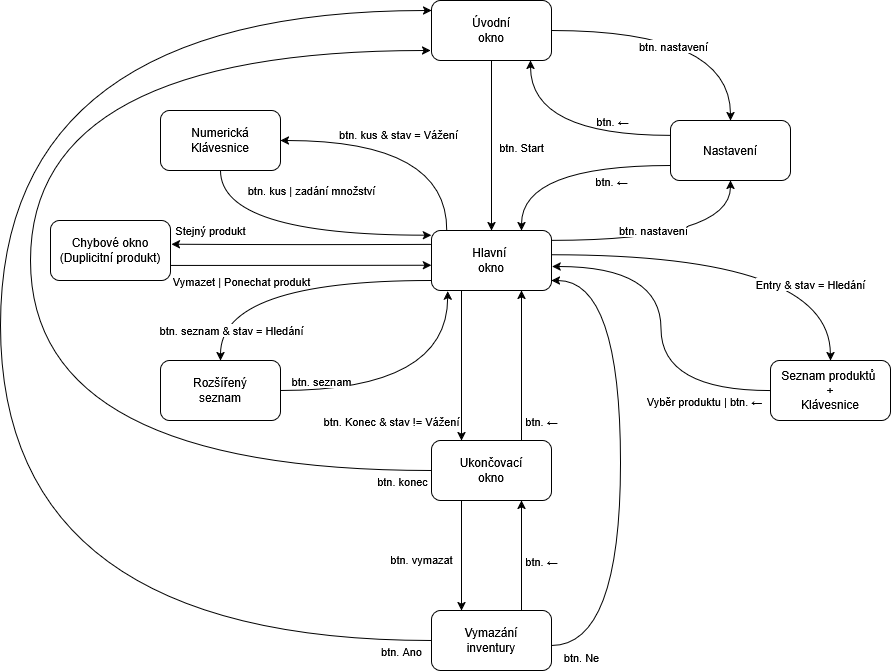
\includegraphics[scale=0.5]{obrazky/Interakce napříč okny GUI.png}
    \end{center}
    \caption{Interakce mezi okny GUI}
    \label{Interakce mezi okny GUI}
\end{figure}

\begin{figure}[H]
    \begin{center}
        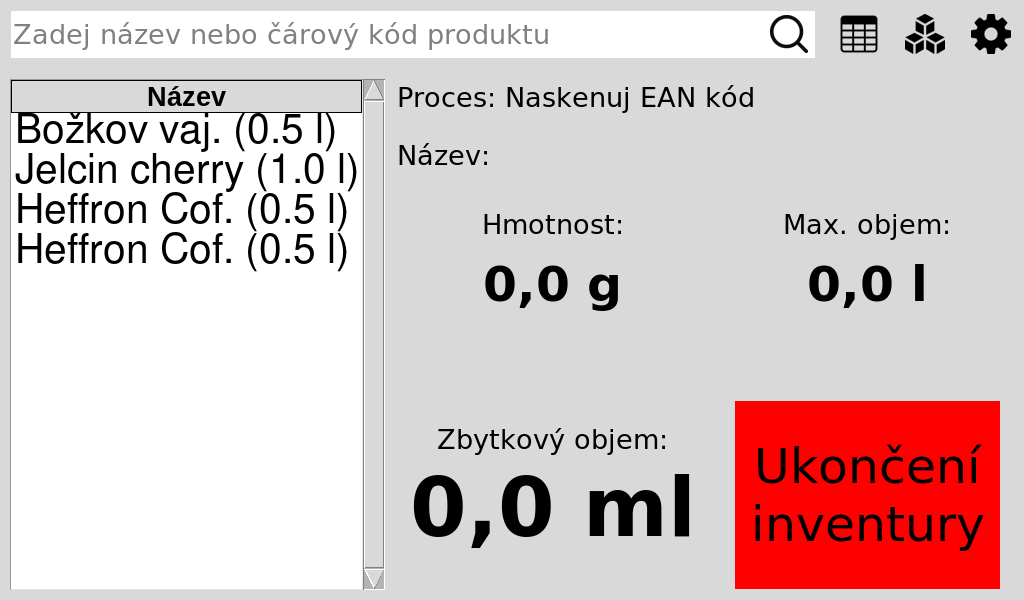
\includegraphics[scale=0.4]{obrazky/GUI Vyhledávání.png}
    \end{center}
    \caption{Hlavní okno ve stavu vyhledávání}
    \label{Interakce mezi okny GUI}
\end{figure}


//OBRAZEK - HL. MENU S PRVKY VE ZKRACENEM SEZNAMU
//Obrázek - komunikace mezi komponentami

\subsection{Proces vyhledání}

%Jak bylo řečeno vyhledání produktu probíhá naskenováním jeho EAN kódu. V přípdě neuspěšného scanu z důvodu poškozeného čárového kódu nebo že daný čárový kód není veden v databázi, systém vypíše do "label_proces" chybové hláčení "[bude doplěno]". V případě, že by byl čárový kód tak moc poškozen, že by nešel přečíst je možnost ho vyhledat ručně pomocí Entry pole. Po kliknutí na Entry pole vyjede seznam (list box) destilátů a ze spodní části obrazovky vyjede klávesnice pro rychlejší vyhledání pomocí zadání názvu.

%nebo ručním vyhledáním pomocí entry(text boxu), kdy po kliknutí na něj nám vyjede seznam se všemi produkty a ve spodní části obrazovky se ukáže klávesnice pro vyhledání

%V tomto stavu jsme schopni už vyhledávat požadovaný produkt buď naskenováním jeho EAN kodu nebo jeho ručním vyhledáním. Pokud se rozhodneme vyhledat produkt pomocí naskenování jeho kodu, ale ten se nepovede najít  případě, že by se nepovedlo vyhledat EAN kod, tak nas aplikace upozorní přes Proces label, že došlo k chybě. V případě ručního vyhledání využijeme Entry(textové pole), kdy na něj stačí kliknout a současně nám vyjede i klávesnice.

Vyhledávání produktu probíhá primárně naskenováním jeho EAN kódu. Pokud je kód nečitelný nebo v databázi neexistuje, zobrazí se chybová hláška [sdsd] v prvku label\_proces. V případě, že je kód natolik poškozený, že jej nelze načíst, je možné produkt dohledat ručně. Kliknutím do vstupního pole (Entry) se zobrazí seznam dostupných destilátů a zároveň se ve spodní části obrazovky otevře klávesnice pro rychlé zadání názvu.

\begin{figure}[H]
    \begin{center}
        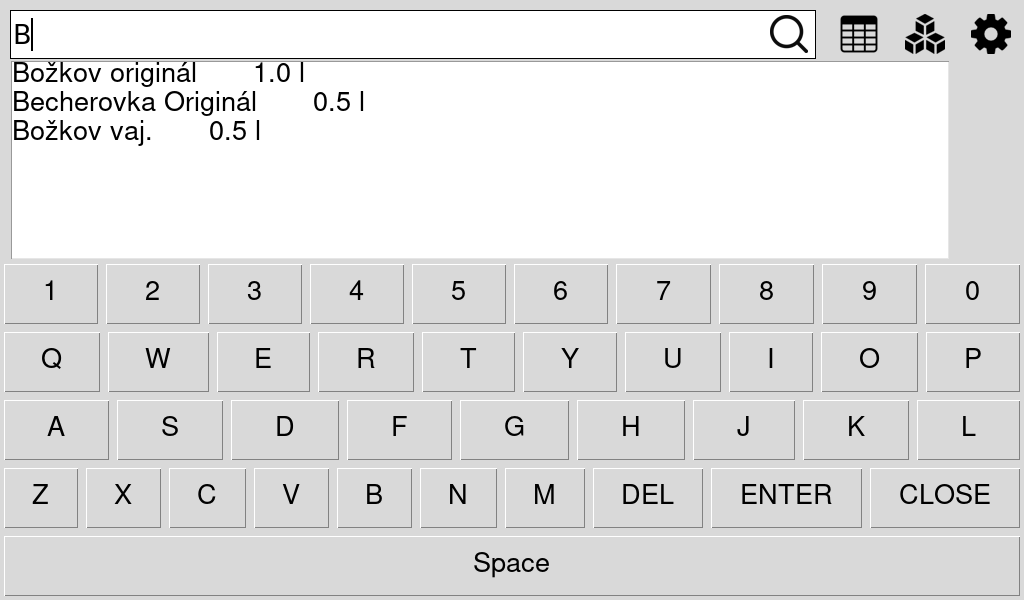
\includegraphics[scale=0.4]{obrazky/GUI Klavesnice + list_box + filr.png}
    \end{center}
    \caption{Hlavní okno - manuální vyhledání produktu}
    \label{Hlavní okno - manuální vyhledání produktu}
\end{figure}
//OBRÁZEK - JAK VYPADÁ RUČNÍ VYHLEDÁNÍ = LISTBOX + KBW

%Do prvku canvas po levé straně se nám začnou ukládat jednotlivé evidované položky ve formě seznamu, kde v závorce za názvem položky máme uvedený jeho maximální objem pro přehled z důvodu kdybysme evidovali stejný druh destilátu, ale v jiné velikosti objemu. V tomto stavu jsme schopni tuto tabulku rozšířit pomocí tlačítka btn. Seznam, kde se nám ukažou podrobné informace jako hmotnost, naměřený objem nebo zadaný počet kusů, taky se nám po pravé straně se nám ukážou tlačítka pro odebraní produktu, snážení/zvýšená počet kusů.

Do seznamu (tree wiev) po levé straně se ukládají již evidované destiláty. V závorce za názvem produktu je uveden jeho maximální objem, což umožňuje odlišit varianty se shodným názvem, ale rozdílnou velikostí balení. Tabulku lze rozšířit kliknutím na tlačítko \texttt{btn.Seznam}, které zobrazí detailní informace jako hmotnost, aktuálně naměřený objem nebo počet evidovaných kusů. Na pravém okraji obrazovky jsou rovněž svisle umístěna ovládací tlačítka pro úpravu množství (přidání/odebrání kusů) a odstranění položky ze seznamu.

\begin{figure}[H]
    \begin{center}
        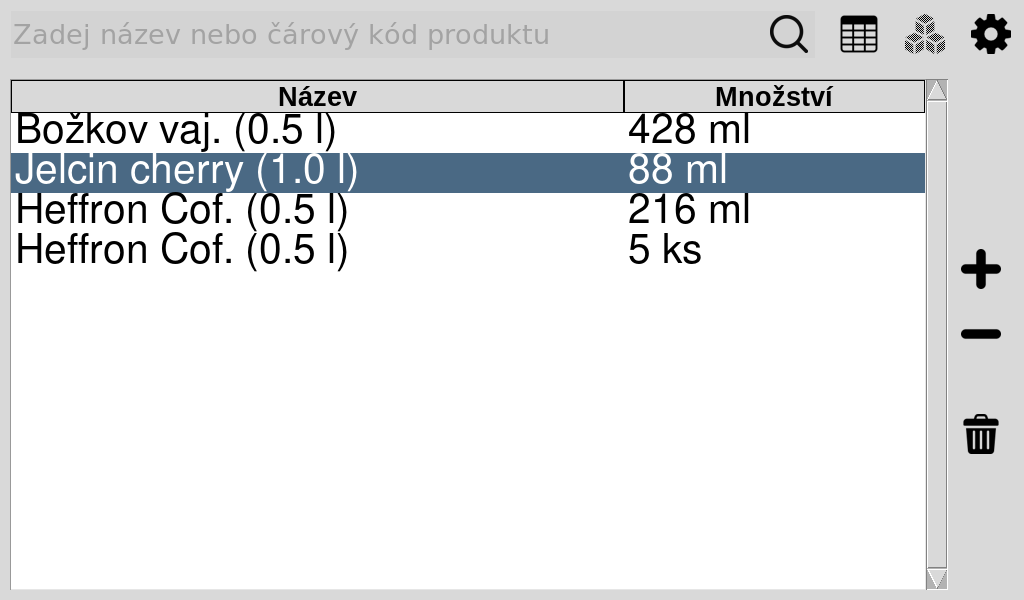
\includegraphics[scale=0.4]{obrazky/GUI Rošířený seznam.png}
    \end{center}
    \caption{Hlavní okno - rozšířený seznam evidovaných produktů}
    \label{Hlavní okno - rozšířený seznam evidovaných produktů}
\end{figure}
//OBRÁZEK - ROZTAŽENÝ SEZNAM

V případě naskenování či vyhledání již evidovaného alkoholu program přejde do stavu "duplicidity".
%Pokud se pokusíme naskenovat nebo ručně vyhledat produkt, který už byl zaevidován, systém automaticky přejde do stavu \textit{duplicity}.


%Nežádoucí stavy:
%\begin{itemize}
%    \item Chyba EAN kódu - Při načtení EAN kódu, který není uložen v databázi nás program upozornění pomocí \textit{proces} labelu, že EAN kod je chybný a ať to zkusíme znovu
%    \item Duplicidní produkt - Pokud se snažíme vyhledat už evidovaný produkt, tak program přejde do stavu duplicidity, tento stav je rozebrán níže. 
%\end{itemize}

\section{Stav - Duplicitní položka}

%Do tohoto stavu jsme se schopni dostat pouze ze stavu vyhledávání a to díky opětovnému vyhledání již evidovaného produktu. V tomto stavu se nám otevře nové okno ve kterém si můžeme vybrat zda zrušíme aktuální výběr(např. kliknutí vedle v seznamu produktů) a vrátíme se do stavu vyhledání nebo produkt budem evidovat i na dále.

Do tohoto stavu se dostaneme pouze prostřednictvím opětovného vyhledání produktu, který již byl jednou zaevidován. Systém následně otevře nové okno, ve kterém má uživatel na výběr: zrušit aktuální výběr (omylem vybral stejný produkt) a vrátit se zpět do stavu vyhledávání, nebo pokračovat do stavu "Vážení".

%\begin{figure}[H]
%    \begin{center}
%        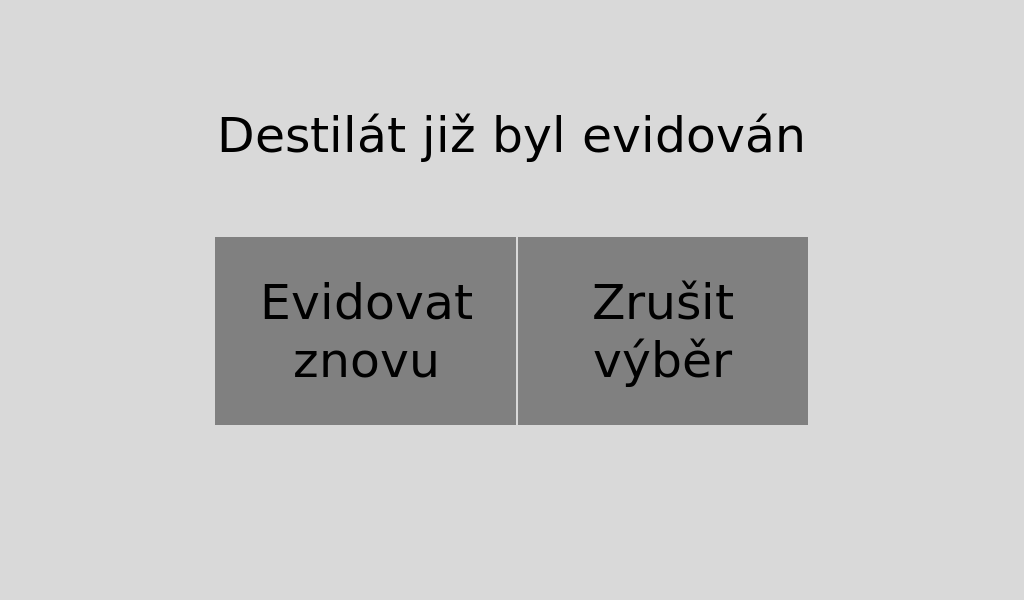
\includegraphics[scale=0.4]{obrazky/GUI Duplicidita.png}
%    \end{center}
%    \caption{Okno informující o duplicitní evidenci produktu}
%    \label{Okno informující o duplicitní evidenci produktu}
%\end{figure}

Opětovná evidence již zaevidovaného produktu má své opodstatnění ve dvou případech:
\begin{itemize}
    \item Pokud máme více rozpitých lahví stejného druhu.
    \item Pokud chceme kromě zbytku z lahve zaevidovat také stav skladu, konkrétně počet neotevřených kusů. K tomu slouží tlačítko pro evidenci kusového zboží s označením btn.stav[xx]
\end{itemize}
%1) Máme více rozpitých lahví
%2) Nechceme evidovat pouze zbytkový objem jedne lahve, ale i stav dané položky ve skladu, tedy počet nenačatých lahví. K tomu slouží tlačítko pro evidenci kusového zboží "btn.stav"[xx]

%Zde muže byt ojeb: Říct že to program hlasí za dvou stavů, když je duplicitní alkohol pouze při zbytkovém objemu ap ak sparatně duplicitní alkohol při kusovém zadávání. Tedy pokud mam alkohol evidovaný pod objemem a chcu ho zadat kusově, tak na tohle nebudu upozorněn protože jsem ho kusově ještě nezadával a to stejný i naopak.

%Chybové hlášení duplicidity:
%Tím, že jsem doposud nechal čtečku běžet v continual modu, tak neustale skenovala a jen při vstrupu od stavu vyhledani jsem čistil vstupní buffer. Ted přepinam mezi countinual a manual režimem, tedy kdžy se dostan do chybové hlašení, tak musím čtečku vypnout protože by četla dal, ale už bych nečistil buffer, takže by se možná hodil novy stav ve kterem bych při zapinal a vypinal čtečku čarovoho kodu, ale to je jen den řadek kodu vlastně no.  

//OBRAZEK - HL. MENU S PRVKY VE ZKRACENEM SEZNAMU
//OBRAZEK - HL. MENU S ROZTAŽENÝM SEZNAMEM
//OBRÁZEK - JAK VYPADÁ RUČNÍ VYHLEDÁNÍ = LISTBOX + KBW
//OBRÁZEK - DUPLICIDITA ZBOŽÍ

\section{Stav - Vážení}
% Obecny popis
Vstupem do tohoto stavu je potvrzena úspěšná identifikace destilátu – buď načtením pomocí EAN kódu, nebo jeho ručním vyhledáním. Zobrazí se detailní informace o daném alkoholickém nápoji:
\begin{itemize}
    \item label Název - Název vyhledaného produktu.
    \item label Hmotnost - Celková hmotnost lahve.
    \item label Max. objem - Maximální objem lahve. Tato informace slouží rozeznat stejný typ destilátu v různých velikostech (0,5 l; 0,7 l; 1 l).
    \item Zbytkový objem - Přepočítaná hmotnost na zbytkový objem v láhvi.
    \item Canvas nyní ukazuje obrázek vybraného produktu. Důvodem je že prodejci, i když né často, mění designe svých lahví a to sebou nese i změnu jejich hmotnosti, v takovém případě je nutné aktualizovat databázi pro daný produkt. U značky a typu lahve \textit{Becherovka originál} (0,5 l) došlo k rozdílu hmotnosti 43 g, díky obměně designu. 
\end{itemize}
\bigskip
Tlačítko pro ukončení inventury se změnilo na "Vrátit zpět" pro případ, že uživatel zvolil špatný produkt.

\begin{figure}[H]
    \begin{center}
        \includegraphics[scale=0.4]{obrazky/GUI Odeberte láhev.png}
    \end{center}
    \caption{Hlavní okno s ukázkou vážení}
    \label{Hlavní okno s ukázkou vážení}
\end{figure}

\subsection{Podmínky vážení}
% Podmínky a omezení - Špatná lahev
Důležitou podmínkou pro správné zvážení je použít správnou láhev. Krom názvu a obrázku produktu je uživatel informován pokud:
\begin{itemize}
    \item \textbf{naměřená hmotnost < hmotnost prázdné láhve} - Proto aby se mohl uložit nově naměřený objem do databáze je nutné, aby naměřená hmotnost byla větší nebo rovna než hmotnost prázdné láhve v opačném případě vyjde objem záporný (na displeji se zobrazí jako nulový) a systém čeká než se hmotnost dostane do požadovaného rozsahu.
    \item \textbf{naměřená hmotnost > hmotnost plné láhve} - V moment kdy je naměřená hmotnost vyšší než hmotnost plné láhve se nám do Proces labelu vypíše chybové hlášení: "a.. Maximální hmotnost plné lahve byla překročena." a Label pro zbytkový objem vypíše: "MAX". V tento moment na váze je položená špatná láhev nebo cizí těleso a systém opětovně čeká než se hmotnost dostane do požadovaného rozsahu.
\end{itemize}

\subsection{Stabilizace váhy}
%Stabilizace váhy
Dalším z důležitých faktorů pro určení finálního naměřeného objemu je stabilizovaná váha. Váha sama o sobě signalizuje svou stabilitu tím, že k posílaným datům přes sériovou linku přidá jednotku hmotnosti [X]. V momentě, kdy je váha stabilizovaná a je v požadovaném rozsahu se text objem uloží do databáze a program se přesune do stavu \textit{"remove\_bottle"}. Uživatel je také o úspěšné stabilizaci váhy informován tím, že pozadí labelu zbytkového objemu se obarví do zelena. 

\subsection{Zadání kusového zboží}
%Zadání kusového zboží
Další z funkcí tohoto systému je evidence neotevřených lahví ve skladu, pomocí tlačítka "kusové zboží" nebo také "sklad". Tato funkce nebyla puvodne zamýšlena, ale po otestování systému v praxi se zjistilo, že je nepraktické některé informace vést do systému (naměřený zbytkový objem) a některé na papír - v praxi to znamená, že člověk krom zbytkového alkoholu uvádí i aktuální stav ve skladu. Proto přibilo toto tlačítko. Po jeho stisknutí se nám oblast s informacemi o zbytkovém objemu (label č1, label č2) překryje numerickou klávesnicí pro zadání počtu kusového zboží. %(možné použít pouze ve stavu vyhledání sortimentu, ale nesmí být aktivovaná rozšířená tabulka)

\begin{figure}[H]
    \begin{center}
        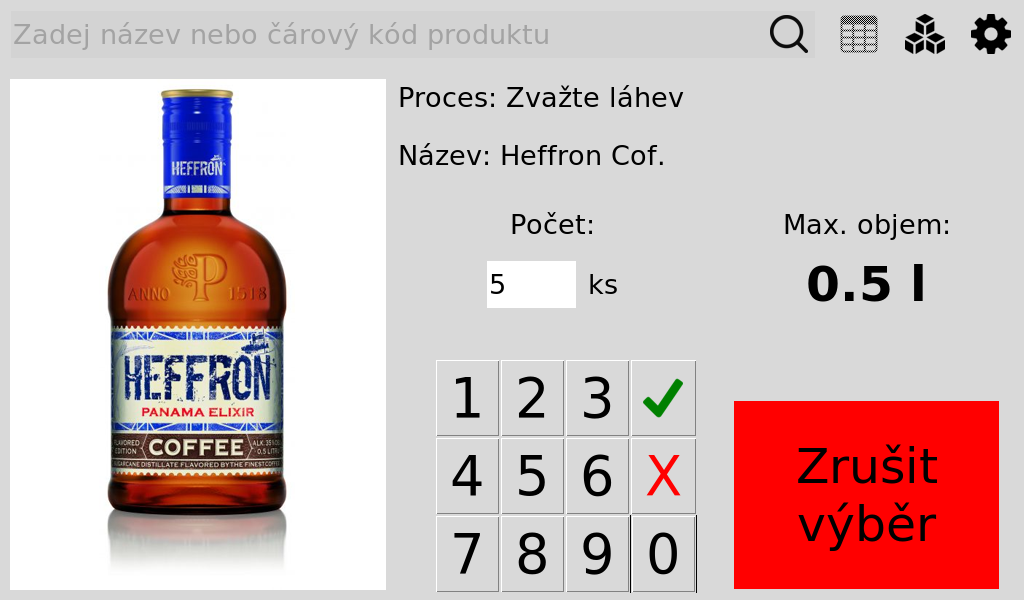
\includegraphics[scale=0.4]{obrazky/GUI Numericka klavesnice.png}
    \end{center}
    \caption{Hlavní okno - zadání kusového zboží ze skladu}
    \label{Hlavní okno - evidence kusového zboží ze skladu}
\end{figure}

%Tato funkce nebyla původně zamýšlená, ale z praktického hlediska jsem ji dodal, protože po otestování systému v praxi vyzněla myš

%\subsection{Použití nalévačů}
% Nevyuití nalévačů
%Další úprava která mě dovedla po otestování systému bylo odstranění původně zamýšlené databáze nalévačů.
%Po otestování systému v praxi se ukázalo, že je nepraktické vést databázi s hmotnostmi různých nalévačů a snažit se převést schopnost v jejich výběru pomocí GUI. Implementace nalévačů do programu, proběhlo dvoumi způsobi:
%1) V hlavním okně jsem vytvořil zaškrtávací políčko, které informovalo zda nalévač je na lahvi či nikoli a každý alkohol měl přidělený ve své databázi svůj nalávač, pokud to bylo nutné změnit přiřazení nalévače dělalo se to přes databázi. bohužel se ukázalo, že s každou inventurou se nalévače na lahvích mění nebo tam nejsou vůbec, proto bylo nepraktické nastavit fixně jeden typ nalevače na jednu láhev. Jednou z možných řešení bylo mít na každou lahev stejný tyto nalévače, ale to pro personal bylo nepraktické a tak je začali sundávat.
%2) Udělal jsem inovaci v tom, že před každou evidenci lahve tedy před jeho navážením zaměstnanec musel vybrat typ nalévače pro danou lahev ze seznamu, který mu vyjel pod Entry oknem, kde bylo přidáno přepínací tlačítko mezi seznamem produktů a nalévačů. Tato metoda se nakonec ukázala jakou zdlouhavá a proto byla odstraněna. Mnohem rychlejší bylo nalévač sthrnout z hrdla lahve a navážit bez něj než ho hledat v seznamu kvuli kompenzaci jeho hmotnosti. Tudíž na základě tohoto všecho jsem odstranil i databázi veškerých nalévačů.

%Po otestování systému v praxi se ukázalo, že je nepraktické vést databázi s hmotnostmi různých nalévačů. V provopočátku některé detiláty měli přiřazený svůj nalévač fixně a uživatel mohl použít zašktrtávací tlačíko pro važení s nalévačem či bez. Bohužel s každou inventurou se nalávače na láhvích pravidelně měnily, proto jsem přidal možnost v uživatli si pro daný alkohol za chodu inventury vybrat ze seznamu konrétní nalévač. Toto řešení se moc neosvědčilo a zaměstnanci raději zvolili vážení bez nalévače a raději ho strhly, protože to pro ně bylo rychlejší než jej hledat v seznamu nebo kontrolovat zda použitý nalévač na láhvi odpovídá nalévači přiřazeného k danému destilátu. Na základě této zkušenosti jsem odebral tuto databázi a možnost vážit s nalévačem. Využití vážení s nalévačem by bylo za předpokladu, že by podnik měl na všechny láhve stejný typ nalévače a nemusel by se zdržovat kontrolou správného typu, pouze voulbou možnosti vážení s nalévačem či bez. Tato řešení se ale neosvěčilo, protože pro zamestnavatele bylo přivětivější nákup nalévačů, které byly zrovna cenově dostupné než řešit nepatrný rozdíl hmotnosti zpusobené špatným nalévačem.


%V tomto stavu nám zbývá navážit zbytkový objem a nebo zadat počet kusů. V tomto satvu jak vidite nam se přejmenovalo tlačítko z ukončení inventury na zpět, tedy mlžeme zrušit náš výběr destilátu v případě chybného zadání ručně např. nebo jsme prostě naskenovali něco co jsme evidovat nechteli.

%//obrazek - vážení destilátu
%//obrázek - zadávání kůsů


\section{Stav - Nastavení aplikace}
Do nastavení se dá dostat v libovolném stavu programu pomocí ozubeného tlačítka. V teto fázi jeste neni dodelane veskre funkce nastavení pouze její vizuál.

Nastavení by mělo poté umožňovat:
Ve finální verzi by nastavení mělo umožňovat:
-Doplneni databaze
-Zpetna kontrola inventury
-nastaveni hesla pro administratorsky pristup
-Nastavení jednotek hmotnosti a objemu
-nastavení jazyku
-nastavení nočního režimu

%\begin{figure}[H]
%    \begin{center}
%        \includegraphics[scale=0.4]{obrazky/GUI Nastavení.png}
%    \end{center}
%    \caption{Okno s nastavením aplikace}
%    \label{Okno s nastavením aplikace}
%\end{figure}


\section{Stav - Konec inventury}

%Pro ukončení inventury je nutné, aby uživatel zadal jméno zaměstnance ze seznamu (dropboxu), kde jsou evidovaní všichni zaměstanci, co můžou vykonávat inventůru, tedy tímto se zaměstnanec podepíše pod svou vlastní inventutu, kterou vykonal, jedná se o bezpečnostní prvek, aby bylo možné v případě nejasností v inventuře dohledat, kdo danou inventuru vykonal. Pokud jmeno nezadáme aplikace nás vyzve k jeho zadání a nepustí nás dál, v opačném případě nás přesměruje na obrazovku, kde se nás zeptá zda jsme si jistí tím, že chceme inventuru ukončit (bezpečností prvkek, kdyby jjsme omilem klikli na ukočení inventury). Po uspěšném ukončení inventury se nám obrazovka přene zpátky na výchozí obrazovku[xx]

%Pro ukončení inventury je nutné, aby uživatel zadal jméno zaměstnance ze seznamu (dropboxu), kde jsou evidovaní všichni zaměstanci, co můžou vykonávat inventůru, tedy tímto se zaměstnanec podepíše pod svou vlastní inventutu, kterou vykonal, jedná se o bezpečnostní prvek, aby bylo možné v případě nejasností v inventuře dohledat, kdo danou inventuru vykonal. Pokud jmeno nezadáme aplikace nás vyzve k jeho zadání a nepustí nás dál. Aktuálně spuštěnou inventuru lze i vymazat např. z důvodu milného spuštění, následně čeká ověřovací okno zda jsem si jistí tímto rozhodnutím. Ať při ukončrní inventury nebo jejího vymazání nás applikace přesměruje zpátky na úvodní obrazovku.

Před samotným ukončením inventury musí uživatel vybrat jméno zaměstnance ze seznamu (rozbalovacího pole), který obsahuje všechny pracovníky oprávněné k provádění inventur. Tento krok slouží jako forma elektronického podpisu – určuje, kdo konkrétní inventuru provedl, což je důležité pro zpětnou dohledatelnost v případě jakýchkoliv nesrovnalostí. Pokud jméno není zadáno, aplikace na tuto skutečnost upozorní a nepovolí pokračovat dále.

V případě, že byla inventura spuštěna omylem, je možné ji zcela vymazat. Před provedením tohoto kroku se zobrazí potvrzovací dialog, který slouží k ověření, zda je uživatel smazáním skutečně jistý.

Po ukončení nebo smazání inventury je uživatel automaticky přesměrován zpět na úvodní okno aplikace (Stav 1).


\begin{figure}[H]
    \begin{center}
        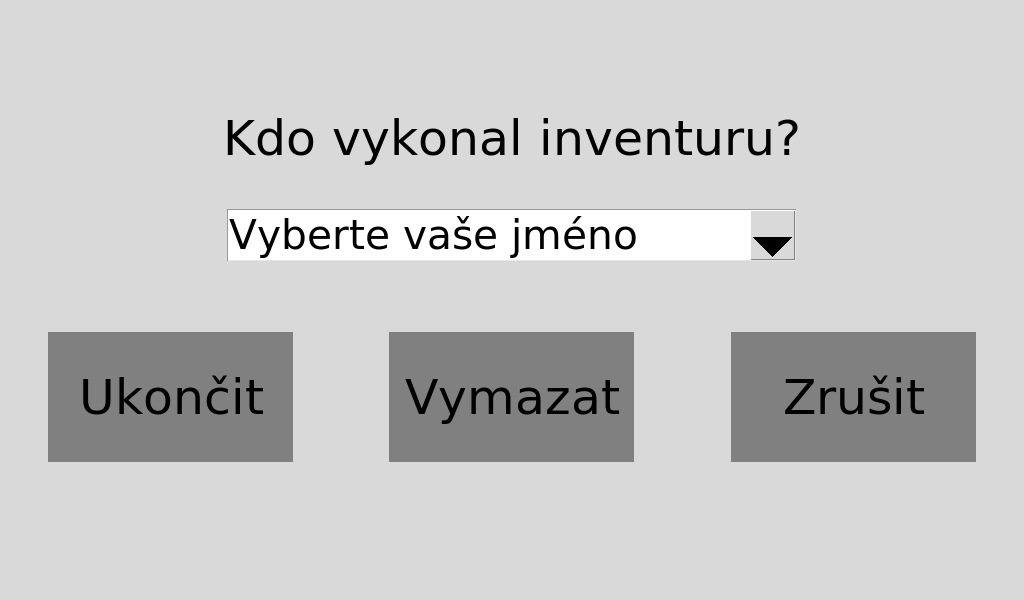
\includegraphics[scale=0.4]{obrazky/GUI Konec inventury.png}
    \end{center}
    \caption{Ukončovací okno aplikace}
    \label{Ukončovací okno aplikace}
\end{figure}

%\begin{figure}[H]
%    \begin{center}
%        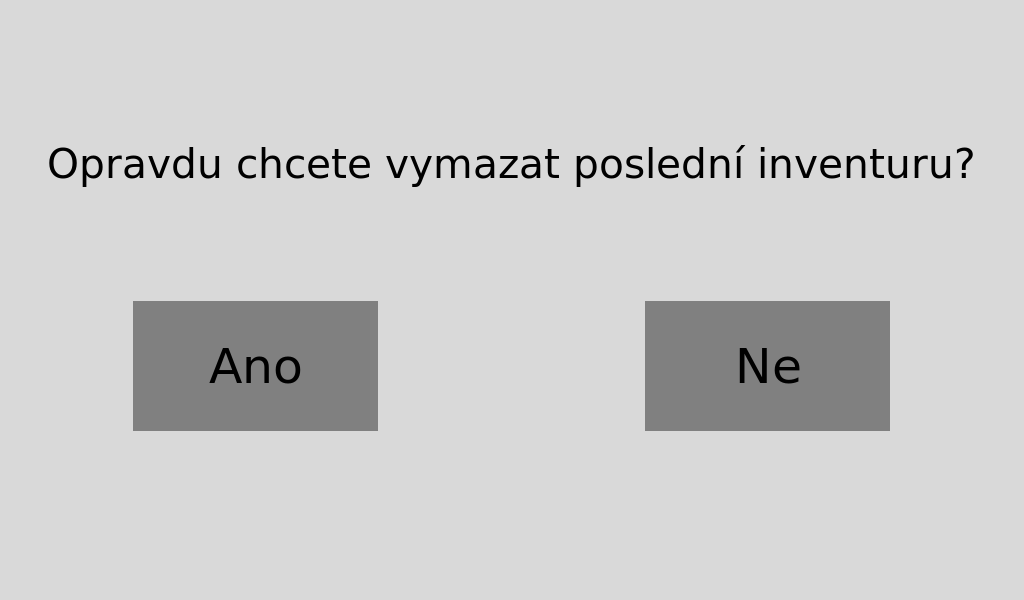
\includegraphics[scale=0.4]{obrazky/GUI Vymazání inventury.png}
%    \end{center}
%    \caption{Potvrzovací okno pro vymazání aktuálně spuštěné inventury}
%    \label{Potvrzovací okno pro vymazání aktuálně spuštěné inventury}
%\end{figure}

\section{Modul grafického prostředí - gui.py}
%V této sekci se zaměříme na programové řešení modulu \texttt{gui.py}. grafické prostředí aplikace je rozděleno do x tříd z důvodu přehlednosti a orientaci v kódu. jedna co ma nastarost vykreslování veškerých oken a další kod, co byl více komplexnejsi, tak jsem zaobalil do vlastní třídy a to třídu pro klavesnici a listbox obsahující seznam destilátů, protože samy o sobě obsahuji dosti kodu, ktery by delal hlavní třídu nepřehlednou. Tyto třídy jsou navzájem provázané pomocí klíčového slova Parent, neboli třida Keyboard a Listbox dědí z hlavní třídy pomocí toho klíčového slova. Parent předává není přímo objekt, je pouze proměná s adresou v paměti na naši hlavní třídu, tedy mužeme skrz toto slovo přistupovat do existujícího objektu.. Nástroj/třída/modul tkinter může vytvořit pouze jedno hlavní okno pomocí klíčového slova tk, tk je třída hlavního okna v programu může být vytvořena jen jednou mé tříde dědím právě ne z třídy, ale modulu..hovno přímo z třídy tk, tudíž mi klíčové slovo self. umožnuje přistupovat k proměným dané třídy tedy i k proměným děděné třídy. tedy pro vytvořeí hlavního okna..ho musím prvně setupunout a pak metodou .mainloop() spusttí hlavní smyčku programu, abych ale mohl komunikovat s dalšími i s jinými třídami a stavovým automatem jako čtečkou a váhou, tak musím z této smyčky i vyskočit, pro tyto účely je metoda after(), proto v mainu ve funkci stavového automatu, opakovaně volám funkci sebe samou

%nevyhodou Pythonu je, že všechny interní proměnné třídy se musí inicializovat uvnitř konstruktoru což v nšem případě, kde máme hromadu ovladacích prvků činí samotnou třídu nepřehlednou a v případě deklarovani promenné v blízkosti metody by se z ní stala statická proměnná. 

%//Ukazka kodu
%Hlavní třída GUI, dědí z třídy Tk, která vytváří hlavní okno programu. V hlavní okno je rozděleno do dvou rámců/framů pro jednoduší vkládání ovládacích prvků. Jedna z metod pro vkládání je grid(), která umožnuje prvky skládat do sloupců a řádku, které mezi sebou interagují a udržují symetrický vzhled. Tudíž třeba když jeden sloupec prvků roztáhnu, ostatní se smrští a prvky se nebudou překrývat přes sebe - dynamické nastavení. Třídy jsou velice rozsáhlé, proto jen vypíchnu to nejduležitějšší.

Táto sekce je zaměřená na programové řešení modulu \texttt{gui.py}. Grafické prostředí aplikace je rozděleno do x tříd z důvodu přehlednosti a orientaci v kódu. Hlavní okno je reprezentováno třídou \texttt{MainWindow}, dědící ze třídy \texttt{Tk}, které spouští hlavní smyčku programu. MainWindow vytváří instanci ostatních tříd, které obsahují kód ostatních oken nebo jinou složitější část kódu. Pro vytvoření nového okna se používá třída \texttt{Toplevel}, které je prostřednictví parametru master přiřazen přídružné okno ke kterému se vztahuje. V případě vyvíjené aplikace jsou všechna Toplevel okna odkázána na hlavní okno. V praxi je spouštěno pouze jedno hlavní okno a libovolný počet Toplevel oken. Jak už bylo jednou zmíněno pro vyskočení z hlavní smyčky za účelem periodických operací(chod stavového automatu, obsluha portů, atd) se využívá metoda after[].

Hlavní okno se skládá ze dvou grafických rámců (tk.Frame) horizontálně rozdělených, kde jeden obsahuje ovládací prvky Entry, a tlačítka pro nastavení, numerickou klávesnici a rozšíření seznamu evidovaných položek. Druhý rámec představuje zbytek okna. Pro vkládání ovládacích prvků do prostředí je využita metoda grid, která umožňuje rozdělit daný rámec na mřížku, kde jednotlivé řádky a sloupce mezi sebou interagují a udržují symetrický vzhled prostředí.



\begin{lstlisting}[language=Python, caption=Funkce stavového automatu, frame=single, breaklines=false]
class MainWindow(tk.Tk):
    def __init__(self):
        super().__init__()
                        ...                       
        self.StartWindow: tk.Toplevel = None
        self.EndWindow: tk.Toplevel = None
        self.SameDest: tk.Toplevel = None
        self.DeleteWindow: tk.Toplevel = None
        self.Settings: tk.Toplevel = None
        self.Keyboard: tk.Toplevel = None
        self.ListBox: tk.Toplevel = None
                        ...
\end{lstlisting}

Ostatní třídy jsou definované stejným způsobem. Ukázka na třídě Keyboard. Třída keyboard dědí ze třídy Toplevel, což je vytváření sekundárních oken GUI, tato třída je provázána s třídou GUI pomocí parametru root. Toplevel, tedy Toplevely mohou odkazovat přímo na hlavní okno nebo jiný Toplevel, předání parametru je pomocí konstruktoru super().\_\_init\_\_(root)

%\begin{lstlisting}[language=Python, caption=Funkce stavového automatu:, frame=single, breaklines=false, postbreak=\mbox{\textcolor{gray}{$\hookrightarrow$}\space}]
%
%class Keyboard(tk.Toplevel):
%    def __init__(self, root:GUI):
%        super().__init__(root)
%        self.root = root
%        self.geometry("1024x600")
%        asd
%        asd
%        as
%        da
%        sd
%        asd
%        as
%        da
%        sda
%        sd
%        asd
%        asd
%        asd
%        
%\end{lstlisting}


\section{Modul databáze - database.py}

Modul \textbf{database.py} zajišťuje trvalé ukládání a vyhledávání údajů o lahvích a inventurních měřeních do relačních databázích \textbf{database.db} a \textbf{inventory.db} uložených lokálně na SD kartě Raspberry Pi. Databáze se dále skládají z tabulek (table) stejně jako Excel se skládá z více listů. Soubory s příponou \textbf{.db} jsou čitelné pro databázový engine SQLite, který umí databázový jazyk SQL. Aby byla práce s daty v Pythonu přehlednější, je využit nástroj (modul) SQLAlchemy:
\begin{itemize}
    \item SQLAlchemy vytváří nad SQLite enginem objektovou vrstvu (ORM).
    \item Každou tabulku mapuje na Python třídu – aplikace tak pracuje s atributy objektů místo ručního skládání příkazů SQL.
    \item Umožňuje jednoduchý přechod na jiný databázový systém (např. \textit{PostgreSQL})
\end{itemize}

\begin{lstlisting}[language=Python,breaklines=false, frame=single, caption=Ukázka třídy database.db a inventory.db]
Chyba latexu
\end{lstlisting}

\subsection{Práce se souborem database.db}
Soubor database.db obsahuje 2 tabulky:
\begin{itemize}
    \item destilate - seznam destilátů a jejich parametry [č.x]
    \item employee\_name - seznam jmen zaměstnanců možných vykonávat inventuru
\end{itemize}
Pro vyhledání konrétního destilátu se používají 2 funkce:
\begin{itemize}
    \item get\_info\_by\_ean - vyhledá produkt na základě jeho EAN kódu
    \item get\_info\_by\_name - vyhledá produkt na základě jeho názvu
\end{itemize}
\begin{lstlisting}[language=Python,breaklines=false, frame=single]
def get_info_by_ean(str:ean) -> Destilate
\end{lstlisting}
\begin{lstlisting}[language=Python,breaklines=false, frame=single]
def get_info_by_name(str:name) -> Destilate
\end{lstlisting}
V obou případech je návratová hodnota \texttt{Destilate} objekt obsahující veškeré informace vyhledaného produktu.
Pro manuální vyhledávání slouží funkce \texttt{get\_rows\_by\_name}, která prohledá tabulku destilátů na základě vloženého substringu a vrátí list polí 2x1 obsahující název destilátu a jeho maximální objem.
\begin{lstlisting}[language=Python,breaklines=false, frame=single]
def get_rows_by_name(substr:str)->list[tuple[str,float]]
\end{lstlisting}

\subsection{Práce se souborem inventory.db}
Databáze inventory.db obsahuje tabulky, které dále obsahují veškeré naměřené data v rámci jedné inventury.

Metoda \texttt{create\_new\_table} je volána po spuštění inventury a úspěšném průchodu stavem \texttt{check\_port} v mainu, kdy vytvoří novou tabulku s názvem inventory a přiřadí jí datum a čas vytvoření pro zpětnou kontrolu. V případě neuspěšného vytvoření tabulky je vyvolána vyjímka \texttt{Exception}.
\begin{lstlisting}[language=Python,breaklines=false, frame=single]
def create_new_inventory_table() -> None
\end{lstlisting}
\bigskip
Metoda rename\_last\_table je volána při ukončení inventury, kdy za konec jména tabulky se přidá jméno pracovníka pro zpětnou kontrolu.
\begin{lstlisting}[language=Python,breaklines=false, frame=single]
def rename_last_table(name:str) -> None
\end{lstlisting}
\bigskip
Poslední funkcí je delete\_last\_table, která vymaže poslední tabulku v inventory.db, např. z důvodu mylného spuštění inventury.
%vytvořenou aktualně běžící inventuru.
\begin{lstlisting}[language=Python,breaklines=false, frame=single]
def delete_last_table() -> None
\end{lstlisting}

%
%\subsection{hledání dat}
%\subsection{výpis dat}
%\subsection{sdsds}




\section{Modul čtečky čárového kódu - sensor.py}
Kamerová čtečka GM65 komunikuje prostřednictvím USBVcom. Čtečka je přepínána mezi čtecími režimi continual a manual viz kapitola č.XXX. 

Kod pro ovládání čtečky je zaobaleno do třídy \texttt{BarcodeSensor} obsažené v modulu \texttt{barcode\_sensor.py}. Třídá dědí ze třídy \texttt{Serial}, která zastřešuje veškerou seriovou komunikaci. Konstruktor třídy BarcodeSensor přebírá parametry pro adresu portu, rychlost seriové komunikace (baudrate) a timeout, který slouží k přerušení zápisu/čtení na daném portu po určitém čase. Tyto veškerý data se následně předají konstruktoru třídy Serial. 

\begin{lstlisting}[language=python,breaklines=true, frame=single]
import serial
class BarcodeSensor(serial.Serial):
    def __init__(self, port=None, baudrate=9600, timeout=1):
        super().__init__(port=port, baudrate=baudrate, timeout=timeout)
\end{lstlisting}
\bigskip
Třída obsahuje metodu \texttt{open\_port}, která otevírá nastavený port pro komunikaci. 
V případě úspěšné otevření vrátí \texttt{True}. 
%Návratovou hodnotou je \texttt{bool} na základě toho, zda se otevření povedlo nebo ne.

\begin{lstlisting}[language=Python,breaklines=false, frame=single]
def open_port(self) -> bool:
\end{lstlisting}

\bigskip
Metoda turn\_on\_sensor přepne čtečku do aktivního stavu, kde se rozsvítí LED dioda, povolí bzučák pro případ naskenování čárového kódu a čtečka přejde do contianul režimu. Opakem této metody je metoda turn\_off\_sensor, kdy čtečka se přepně do manuálního režimu. Předpis datového packetu odesilaného do čtečky se skládá z:

\begin{itemize}
    \item hlavička (head) - Značí odesílatele dat (0xEA 0x00: řídící jednotka → čtečka)
    \item Zone byte (types) – Typ operace (zápis do čtečky, výpis nastavení, ...)
    \item lens – délka bloku \textit{data} v bajtech
    \item adress – oblast nastavení (typ čtení, rychlost čtení, typ kódu)
    \item data – konkrétní nastavení dané oblasti (zapnutí LED diody, čtecí režim, ...)
    \item CRC – kontrolní součet (XOR) detekující chybnou zprávu. 
\end{itemize}

\begin{table}[H]
    \centering
    \begin{tabular}{|c|c|c|c|c|c|}
         \hline
         Head & Types & Lens & Adress & Data & CRC\\ \hline
         0x7E 0x00 & 0x08 & 0x01 & 0x00 0x00 & 0xEA & 0x?? 0x??\\
         \hline
    \end{tabular}
    \caption{Předpis datového packetu pro aktivaci čtečky}
    \label{tab:my_label}
\end{table}

\begin{table}[H]
    \centering
    \begin{tabular}{|c|c|c|}
         \hline
         Pořadí bitu & Hodnota bitu & Funkce \\ \hline
         7. & 1 & Probliknutí při přečtení kódu \\ \hline
         6. & 1 & Zapnutí bzučáku \\ \hline
         5-4. & 10 & Nastaví se stejně jako 2-3. bit \\ \hline
         3-2. & 10 & Zapnutí LED \\ \hline
         1-0. & 10 & Continual mode (Čtecí režim)\\ \hline
    \end{tabular}
    \caption{Výpis funkcí jednotlivých bitů bloku "Data". 0xEA (HEX) = 11101010 (binary)}
    \label{tab:my_label}
\end{table}

%\begin{lstlisting}[language=Python, caption=Metoda turnooonoosensor, frame=single, breaklines=false, postbreak=\mbox{\textcolor{gray}{$\hookrightarrow$}\space}]
%
%def turn_on_sensor(self) -> bool:
%
%    data_on = bytes([0x08, 0x01, 0x00, 0x00, 0xEA])
%    crc_on = self.crc16_ccitt(data_on)
%    crc_on_high = (crc_on >> 8) & 0xFF
%    crc_on_low = crc_on & 0xFF
%           
%    scan_command:bytes = bytes([0x7E, 0x00]) + data_on + bytes([crc_on_high, crc_on_low])
%    self.write(scan_command)
%    ack:bytes = self.read(7)
%
%    if ack == bytes([0x02, 0x00, 0x00, 0x01, 0x00, 0x33, 0x31]):
%        return True
%    else:
%        return False
%\end{lstlisting}
\bigskip
Metoda \texttt{crc16\_ccitt} vykonává kontrolní 16 bitový součet z bloků \textit{Types} až \textit{Data}. Výstupem je 16 bitové číslo, které je následně rozděleno na 2 separátní bajty.[zdroj1]
%https://srecord.sourceforge.net/crc16-ccitt.html

%\begin{lstlisting}[language=Python,breaklines=false, frame=single,postbreak=\mbox{\tiny$\hookrightarrow$}]
%
%def crc16_ccitt(self, data: bytes, poly=0x1021, crc=0x0000) -> int:
%    for byte in data:
%        crc ^= (byte << 8)
%        for _ in range(8):
%            if (crc & 0x8000):
%                crc = ((crc << 1) ^ poly) & 0xFFFF
%            else:
%                crc = (crc << 1) & 0xFFFF
%\end{lstlisting}
\bigskip
Jako poslední metoda je \texttt{read\_sensor\_data} která posílá nazpět naskenovaná data uložená ve vstupním bufferu mikropočítače.
%\begin{lstlisting}[language=Python,breaklines=false, frame=single,postbreak=\mbox{\tiny$\hookrightarrow$}]
%
%def read_sensor_data(self) -> str:
%    if self.in_waiting == 0:
%        return ''
%    return self.read(15).decode()
%\end{lstlisting}

\section{Modul váhy - scale.py}
Digitální váha G\&G E3000 komunikuje po linkách TX/RX standardu RS‑232 ve formátu 8 N 1 a baudrate 9600 Bd. Aby bylo možné váhu připojit k jednodeskovému počítači Raspberry Pi 4, je rozhraní převáděno adaptérem AXAGO ADS‑50 na virtuální COM port USB CDC (obr. 6‑3). Pro tuto váhu byla vytvořena třída Scale zastřešující veškero serivou komunikaci váhy s mikropočítačem. Konstruktor třídy přebírá parametry pro nastavení portu, baudrate a timeout který nastavuje, čtení na seriovém portu po dobu 1 s. Pokud do tohoto intervalu nejsou zaznamenány žádné příchozí data, čtení se ukončí. Třída dále dědí ze třídy serial, které předává všechny zmíněné parametry.

\begin{lstlisting}[language=Python,breaklines=false, frame=single]
class Scale(serial.Serial):
    def __init__(self) -> None:
        super().__init__(baudrate = 9600, timeout=1)
\end{lstlisting}

\subsection{Ověření komunikace s váhou}
Aby bylo možno s váhou komunikovat je nutné otevřít port na kterém je připojena a to pomocí metody \texttt{open\_port}, která je volána z druhého stavu v mainu. V případě chyby se vyvolá výjimka xxxa a metoda vrátí \texttt{False}.

\begin{lstlisting}[language=Python,breaklines=false, frame=single]
def open_port(self) -> bool:
\end{lstlisting}

Po úspěšném otevření portu se zkontroluje zda váha komunikuje (není vypnutá) pomocí metody \texttt{check\_conection} tím že pošle příkaz \textbf{0xBH 0x70} a váha odpoví kolik navážila, předpis ACK zprávy je ve tvaru [sss].

\begin{lstlisting}[language=Python,breaklines=false, frame=single]
def check_conection(self) -> bool:
\end{lstlisting}

\subsection{Komunikace s váhou po sériové lince}

Ke komunikaci slouží metoda  \texttt{print\_scale}, která odesílá stejnou zprávu jako metoda \texttt{check\_conection}, pokud ale váha neodpoví do stanoveného času pomocí timeoutu zkontroluje se zda je port otevřený, pokud není metoda vrátí \textit{Err1} a pokud je metoda vrátí \textit{Err0}.

\begin{lstlisting}[language=Python,breaklines=false, frame=single]
def print_scale(self) -> str:
\end{lstlisting}
Problém je že váha neposílá žádný kontrolní znak a ani neobsahuje paritu, proto abychom se ujistili, že příchozí data nejsou poškozena budem kontrolovat zda poslední 3 přijaté zprávy jsou shodné dle stavového diagramu \ref{ošetření parity}. Kontrolovat budem pouze zprávy které došli s jednotkou hmotnosti, čímž váha říká, že je stabilizovaná. Důvodem je, že pokud zatížíme váhu, tak její naměřená hmotnost se velice rychle mění, proto bysme nedokázali přijmout v této fázi 2 stejné hodnoty hmotnosti posobě v rámci kodu jsou zpracovávána pouze stabilizovaná data.

%% NÍŽE VYMAZAT VŠE

%%stavák ošetření stavového automatu
%\begin{figure}[H]
%    \begin{center}
%        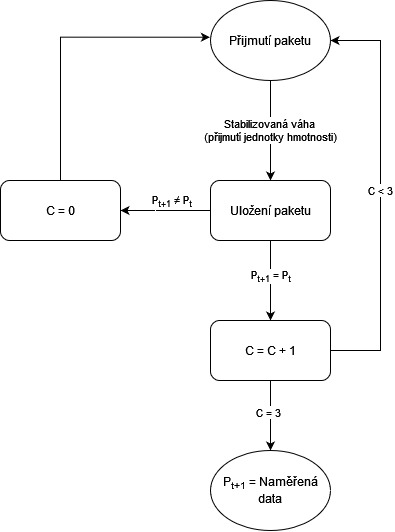
\includegraphics[scale=0.6]{obrazky/stavovy_automat_parita.jpg}
%    \end{center}
%    \caption{Kontrola příchozích zpráv z váhy}
%    \label{ošetření parity}
%\end{figure}
%
%
%navíc do databáze se ukládají až stabilizované hodnoty, proto
%
%
%
%
%Tok dat směřuje obousměrně – váha odesílá měřené hodnoty, řídicí jednotka je v intervalech \~200 ms vyžaduje řídicím párem znaků ESC 'p'. Třída Scale zastřešuje veškero serivou komunikaci váhy s Raspberry Pi. Třída dědí ze třídy Serial, kde v jejím konstruktoru nastavujeme baudrate 9600 a timeout=5s. 
%
%Metoda open\_port() je volána z druhého stavu v mainu, která otevírá serivový port pro komunikaci v případě selhání vyhodí vyjímku vrátí hodnotu False.
%
%Dále je metoda check\_conection(), která se volá po uspěšnem otevření portu a kontroluje zda váha komunikuje, tím že pošle příkaz na ve tvaru esc+p a váha odpoví kolik navážila, pokud jsou data přijata (je jedno co pošle), tak váha komunikuje.
%
%Nejduležitší metodou je print\_scale(), která odesílá požadavek na "tisk" dat. Tím, že váha neposílá paritní bit, děláme SW kontrolu, zda 3 poslední zprávy jsou shoné pomocí stavového diagramu obrč.x
%
%\begin{lstlisting}[language=Python, caption=Funkce stavového automatu:, frame=single]
%def print_scalee(self) -> str:
%\end{lstlisting}

\section{Spouštěcí script}
\section{Splash obrazovka}
\section{Praktická úkázka}
Hodit sem fotku celého systému

Pak sem hodit fotku malého odměrného válce s vysokou přesností a porovnat to s fotkou kde jsem navážil stejný objem - at jde vydet hlavne lahev na váze + displej váhy, pak celý displej, jestli ukazuje stejnou hmotnost + nove vypočítaný objem.

Mozna udelat aj nejaký výpočet